\documentclass[a5paper, 10pt]{article}

% Текст
\usepackage[utf8]{inputenc} % UTF-8 кодировка
\usepackage[russian]{babel} % Русский язык
\usepackage{indentfirst} % красная строка в первом параграфе в главе
% Отображение страниц
\usepackage{geometry} % размеры листа и отступов
\usepackage{listings}
\usepackage{color}

\geometry{
	left=12mm,
	top=25mm,
	right=15mm,
	bottom=17mm,
	marginparsep=0mm,
	marginparwidth=0mm,
	headheight=10mm,
	headsep=7mm,
	nofoot}
\usepackage{afterpage,fancyhdr} % настройка колонтитулов
\pagestyle{fancy}
\fancypagestyle{style}{ % создание нового стиля style
	\fancyhf{} % очистка колонтитулов
	\fancyhead[LO, RE]{Лабораторная работа № 3 } % название документа наверху
	\fancyhead[RO, LE]{Жёсткая фильтрация} % название section наверху
	\fancyfoot[RO, LE]{\thepage} % номер страницы справа внизу на нечетных и слева внизу на четных
	\renewcommand{\headrulewidth}{0.25pt} % толщина линии сверху
	\renewcommand{\footrulewidth}{0pt} % толцина линии снизу
}
\fancypagestyle{plain}{ % создание нового стиля plain -- полностью пустого
	\fancyhf{}
	\renewcommand{\headrulewidth}{0pt}
}
\fancypagestyle{title}{ % создание нового стиля title -- для титульной страницы
	\fancyhf{}
	\fancyhead[C]{{\footnotesize
			Министерство образования и науки Российской Федерации\\
			Федеральное государственное автономное образовательное учреждение высшего образования
	}}
	\fancyfoot[C]{{\large 
			Санкт-Петербург, 2024
	}}
	\renewcommand{\headrulewidth}{0pt}
}

% Математика
\usepackage{amsmath, amsfonts, amssymb, amsthm} % Набор пакетов для математических текстов
%\usepackage{dmvnbase} % мехматовский пакет latex-сокращений
\usepackage{cancel} % зачеркивание для сокращений
% Рисунки и фигуры
\usepackage[pdftex]{graphicx} % вставка рисунков
\usepackage{wrapfig, subcaption} % вставка фигур, обтекая текст
\usepackage{caption} % для настройки подписей
\captionsetup{figurewithin=none,labelsep=period, font={small,it}} % настройка подписей к рисункам
% Рисование
\usepackage{tikz} % рисование
\usepackage{circuitikz}
\usepackage{pgfplots} % графики
% Таблицы
\usepackage{multirow} % объединение строк
\usepackage{multicol} % объединение столбцов
% Остальное
\usepackage[unicode, pdftex]{hyperref} % гиперссылки
\usepackage{enumitem} % нормальное оформление списков
\setlist{itemsep=0.15cm,topsep=0.15cm,parsep=1pt} % настройки списков
% Теоремы, леммы, определения...
\theoremstyle{definition}
\newtheorem{Def}{Определение}
\newtheorem*{Axiom}{Аксиома}
\theoremstyle{plain}
\newtheorem{Th}{Теорема}
\newtheorem{Lem}{Лемма}
\newtheorem{Cor}{Следствие}
\newtheorem{Ex}{Пример}
\theoremstyle{remark}
\newtheorem*{Note}{Замечание}
\newtheorem*{Solution}{Решение}
\newtheorem*{Proof}{Доказательство}
% Свои команды
\newcommand{\comb}[1]{\left[\hspace{-4pt}\begin{array}{l}#1\end{array}\right.\hspace{-5pt} } % совокупность уравнений
% Титульный лист
\usepackage{csvsimple-l3}
\newcommand*{\titlePage}{
	\thispagestyle{title}
	\begingroup
	\begin{center}
		%		{\footnotesize
			%			Министерство образования и науки Российской Федерации\\
			%			Федеральное государственное автономное образовательное учреждение высшего образования
			%		}
		%		
		\vspace*{6ex}
		
		{\small
			САНКТ-ПЕТЕРБУРГСКИЙ НАЦИОНАЛЬНЫЙ ИССЛЕДОВАТЕЛЬСКИЙ УНИВЕРСИТЕТ ИТМО	
		}
		
		\vspace*{2ex}
		
		{\normalsize
			Факультет систем управления и робототехники
		}
		
		\vspace*{15ex}
		
		{\Large \bfseries 
			Лабораторная работа № 3
		}
\vspace*{2ex}
	{\Large \bfseries 
			
"Жёсткая фильтрация"
		}
\vspace*{2ex}
		
		{\normalsize
			по дисциплине Частотные методы
		}

	\end{center}
	\vspace*{20ex}
	\begin{flushright}
		{\large 
			\underline{Выполнила}: студентка гр. \textbf{R3238}\\
			\begin{flushright}
				\textbf{Нечаева А. А.}\\
			\end{flushright}
		}
		
		\vspace*{5ex}
		
		{\large 
			\underline{Преподаватель}: \textit{Перегудин Алексей Алексеевич}
		}
	\end{flushright}	
	\newpage
	\setcounter{page}{1}
	\endgroup}

\begin{document}
	\titlePage
	\pagestyle{style}
\newpage

\section{Задание. Жёсткие фильтры.}
Зададимся числами $a = 1$, $t_1 = 0$, $t_2 = 2$ такими, что $t_1 < t_2$, и рассмотрим функцию $g$ такую, что $g(t) = a$ при $t \in [t_1, t_2]$ и $g(t) = 0$ при других $t$.\\
\\
 Выберем большой интервал $T = 20$ и маленький шаг дискретизации $dt$, соответствующий разбиению рассматриваемого интервала на 1000 точек. Зададим массив времени на отрезке $t = [-T/2,T/2]$ и найдем массив значений $g$ рассматриваемой функции на множестве точек $t$. Зададим зашумленную версию сигнала как
$$u = g + b \cdot (rand(size(t))-0.5) + c \cdot \sin (d \cdot t)$$

Выполним жёсткую фильтрацию указанного сигнала. Для выполнения фильтрации будем поступать так: будем находить Фурье-образ сигнала $u$, затем обнулять его значения на некоторых (выбранных нами) диапазонах частот, затем восстанавливать сигнал с помощью обратного преобразования.


\begin{figure}[h]
\center{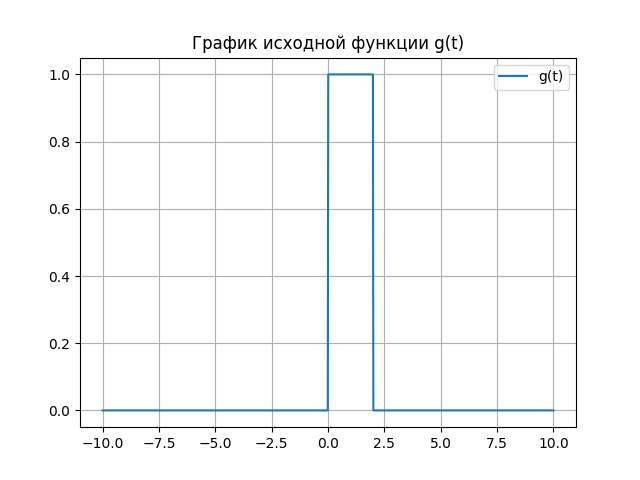
\includegraphics[width=0.8\linewidth]{pic/g_orig.png}}
\caption{График исходной функции $g(t)$.}
\end{figure}

\begin{figure}[h]
\center{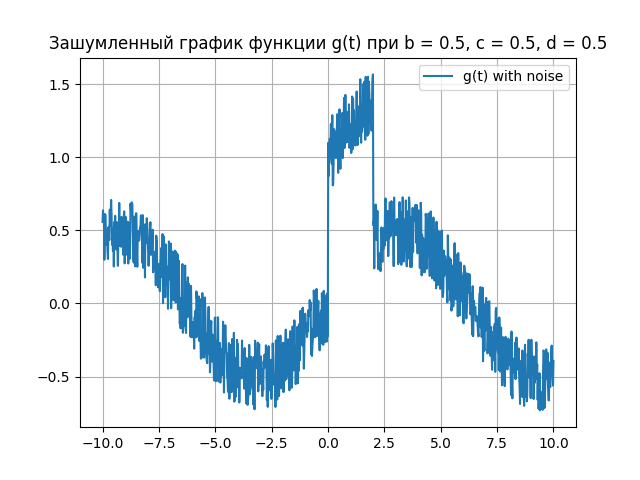
\includegraphics[width=0.7\linewidth]{pic/n_0.5_0.5_0.5.png}}
\caption{График функции $g(t)$ с шумами при $b = 0.5, c = 0.5, d = 0.5$.}
\end{figure}

\subsection{Убираем высокие частоты}

\begin{figure}[h!]
\center{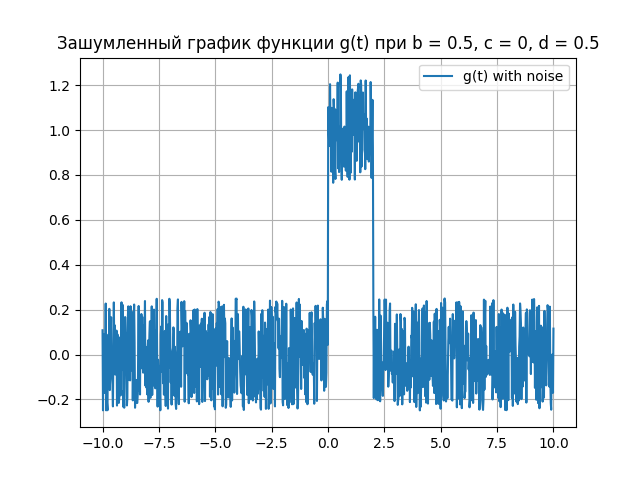
\includegraphics[width=0.7\linewidth]{pic/n_0.5_0_0.5.png}}
\caption{График функции $g(t)$ с шумами при $b = 0.5, c = 0, d = 0.5$.}
\end{figure}

График с шумами при $c= 0$ представлен на рисунке 3. \\
Найдем Фурье-образ сигнала $u$.
\begin{equation}
\hat{f}(\omega) = \frac{1}{\sqrt{2 \pi}} \int_{-\infty}^{\infty} f(t) e^{-i t \omega} dt
\end{equation}

\begin{figure}[h!]
\center{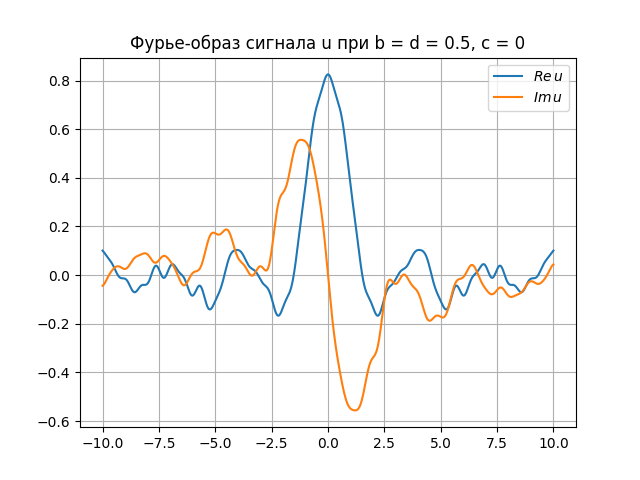
\includegraphics[width=1\linewidth]{pic/f_im_0.5_0_0.5.png}}
\caption{Фурье-образ функции $u(t)$ при $b = 0.5, c = 0, d = 0.5$.}
\end{figure}

Частоту мы определили так: $V = 1 / dt = 1000 / 20 = 50$ $-$ ширина диапазона частот, $dv = 1 / T = 1 / 20$ $-$ шаг частоты.\\

Оставим неизменным Фурье-образ для диапазона частот $[-\nu_0, \nu_0]$ и обнулим его значения на всех остальных частотах. Пусть $\nu_0 = 8$. Результат предствлен на рисунке 5.

\begin{figure}[h!]
\center{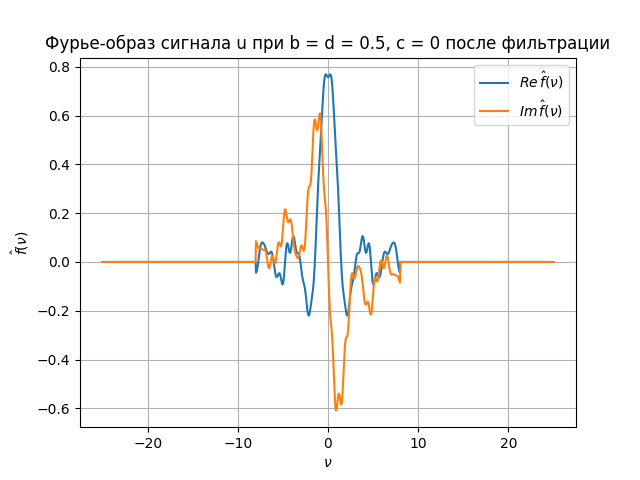
\includegraphics[width=1\linewidth]{pic/f_im_0.5_0_0.5_filter88.png}}
\caption{Фурье-образ функции $u(t)$ при $b = 0.5, c = 0, d = 0.5$ после обнуления.}
\end{figure}



\newpage
Теперь выполним обратное преобразование Фурье для полученного графика. \\
Формула для обратного преобразования Фурье:
\begin{equation}
  f(t) = \frac{1}{\sqrt{2 \pi}} \int_{-\infty}^{\infty}\hat{f}(\omega) e^{i t \omega} d \omega
\end{equation}

\begin{figure}[h!]
\center{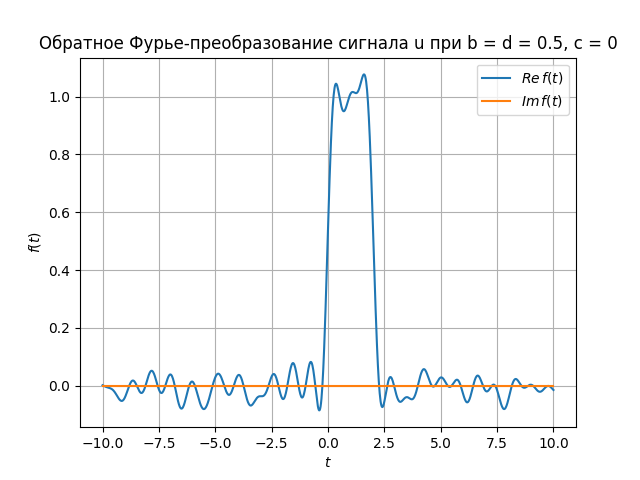
\includegraphics[width=1\linewidth]{pic/f_ift_0.5_0_0.5.png}}
\caption{Обратное Фурье-преобразование функции $u(t)$ при $b = 0.5, c = 0, d = 0.5$ после фильтрации.}
\end{figure}


\begin{figure}[h]
\begin{minipage}[h]{0.5\linewidth}
\center{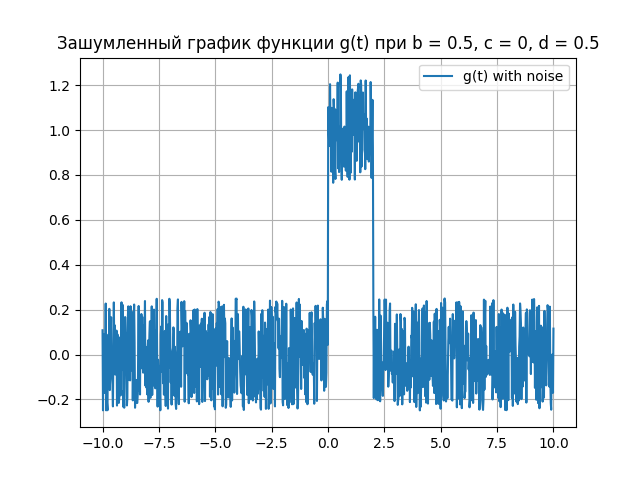
\includegraphics[width=1\linewidth]{pic/n_0.5_0_0.5.png}\\а)}
\end{minipage}
\hfill
\begin{minipage}[h]{0.5\linewidth}
\center{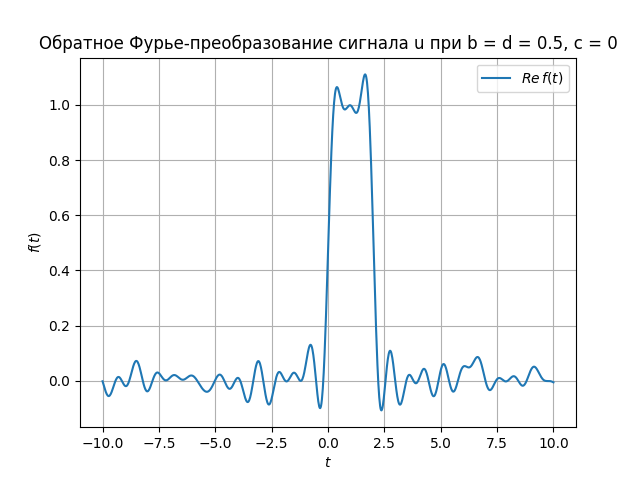
\includegraphics[width=1\linewidth]{pic/ift_0.5_0_0.5.png}\\б)}
\end{minipage}
\caption{Сигнал $u(t)$ до фильтрации высоких частот(а) и после(б).}
\end{figure}

\newpage
На рисунках 6 и 7 хорошо заметно, что полученный после фильтрации график менее зашумлен.\\
\\
Рисунок 8 иллюстрирует близость исходной функции к полученному после фильтрации высоких частот зашумленному графику.


\begin{figure}[h!]
\center{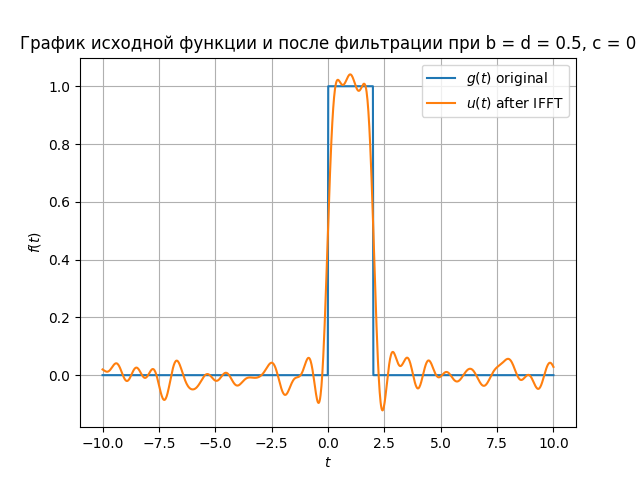
\includegraphics[width=0.9\linewidth]{pic/or_fil_0.5_0_0.5.png}}
\caption{Исходная функция $g(t)$ при $b = 0.5, c = 0, d = 0.5$  и после очистки зашумленного сигнала.}
\end{figure}




\newpage


Построим сравнительные графики модуля Фурье-образа исходного и фильтрованного сигналов.


\begin{figure}[h!]
\center{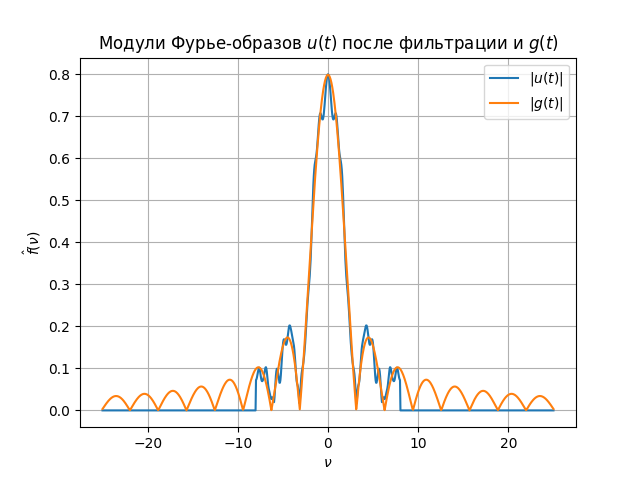
\includegraphics[width=0.9\linewidth]{pic/abs_0.5_0_0.5.png}}
\caption{Сравнительные графики модуля Фурье-образа исходного и фильтрованного сигналов при $b = 0.5, c = 0, d = 0.5$.}
\end{figure}

Исследуем влияние частоты среза $\nu_0$ и значения параметра $b$ на эффективность фильтрации. \\

Пусть $\nu_0 = [4, 8, 10]$, $b = [0.1, 0.25, 0.5, 1]$.



\begin{figure}[h!]
\begin{minipage}[h]{0.5\linewidth}
\center{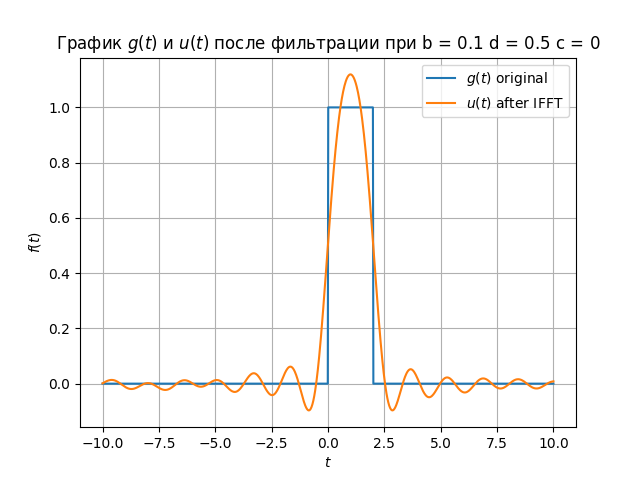
\includegraphics[width=1\linewidth]{pic/f_0.1_4.png}\\а)}
\end{minipage}
\hfill
\begin{minipage}[h]{0.5\linewidth}
\center{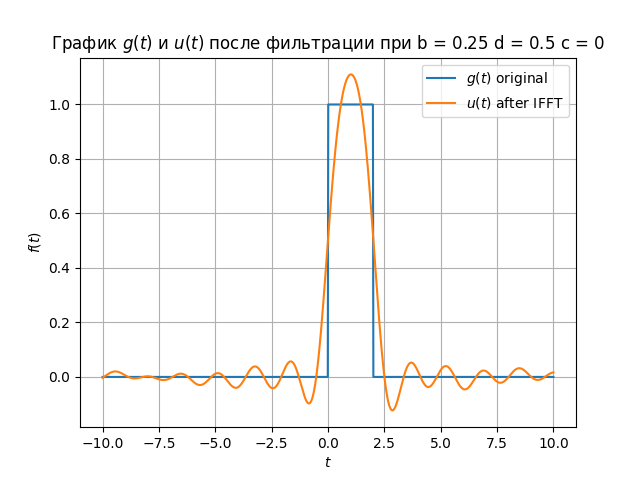
\includegraphics[width=1\linewidth]{pic/f_0.25_4.png}\\б)}
\end{minipage}
\caption{Сигнал $g(t)$ и $u(t)$ после фильтрации при $\nu_0 = 4$ а) $b=0.1$, б) $b=0.25$.}

\begin{minipage}[h]{0.5\linewidth}
\center{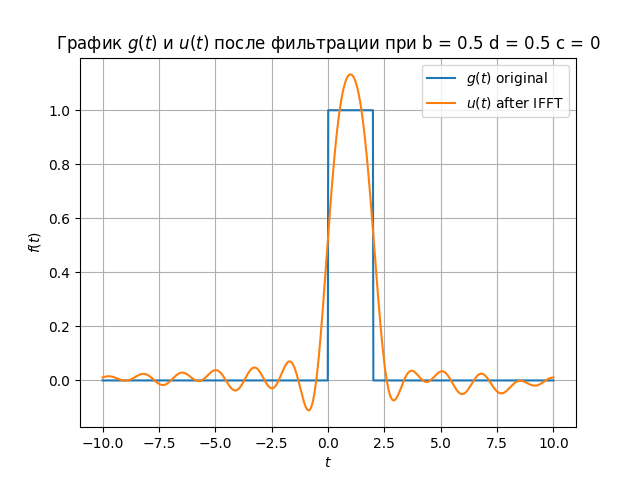
\includegraphics[width=1\linewidth]{pic/f_0.5_4.png}\\а)}
\end{minipage}
\hfill
\begin{minipage}[h]{0.5\linewidth}
\center{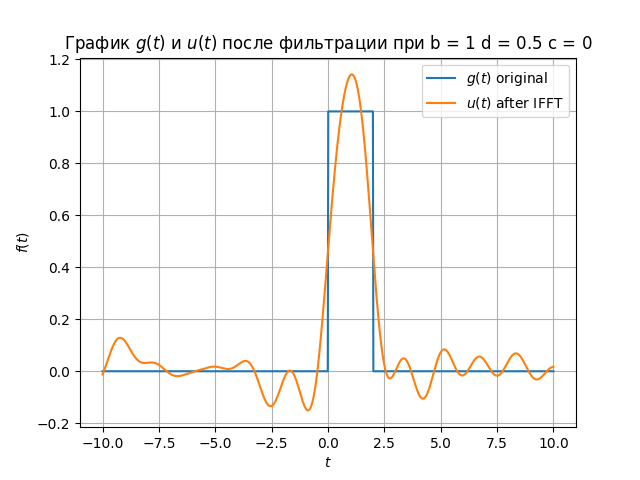
\includegraphics[width=1\linewidth]{pic/f_1_4.png}\\б)}
\end{minipage}
\caption{Сигнал $g(t)$ и $u(t)$ после фильтрации при $\nu_0 = 4$ а) $b=0.5$, б) $b=1$.}
\end{figure}

\newpage
При анализе графиков с одинаковой частотой, но разным коэффициентом $b$, можно заметить,  незначительно эффективнее прошла фильтрации при наименьшем значении $b$ (рисунки 10-11).

\begin{figure}[h!]
\begin{minipage}[h]{0.5\linewidth}
\center{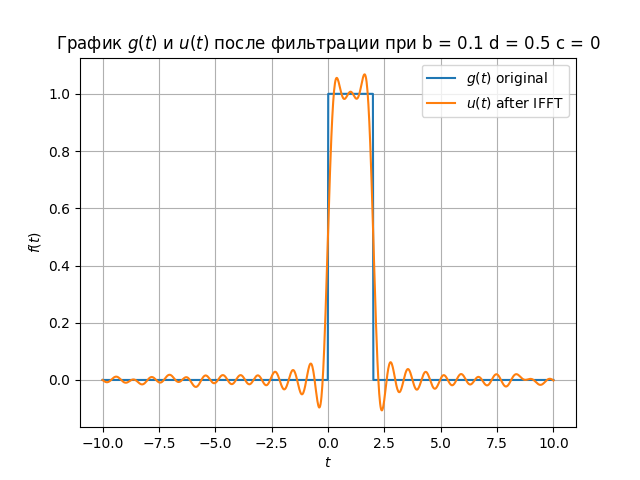
\includegraphics[width=1\linewidth]{pic/f_0.1_8.png}\\а)}
\end{minipage}
\hfill
\begin{minipage}[h]{0.5\linewidth}
\center{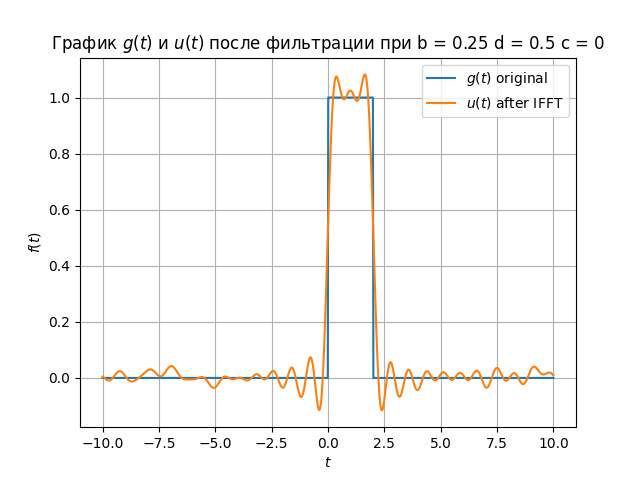
\includegraphics[width=1\linewidth]{pic/f_0.25_8.png}\\б)}
\end{minipage}
\caption{Сигнал $g(t)$ и $u(t)$ после фильтрации при $\nu_0 = 8$ а) $b=0.1$, б) $b=0.25$.}

\begin{minipage}[h]{0.5\linewidth}
\center{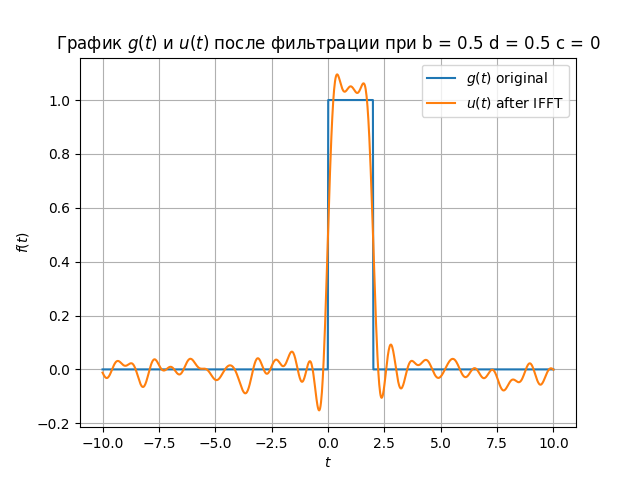
\includegraphics[width=1\linewidth]{pic/f_0.5_8.png}\\а)}
\end{minipage}
\hfill
\begin{minipage}[h]{0.5\linewidth}
\center{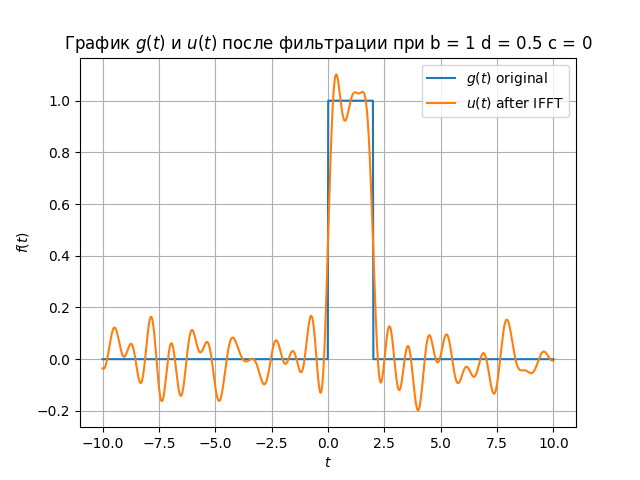
\includegraphics[width=1\linewidth]{pic/f_1_8.png}\\б)}
\end{minipage}
\caption{Сигнал $g(t)$ и $u(t)$ после фильтрации при $\nu_0 = 8$ а) $b=0.5$, б) $b=1$.}
\end{figure}


\newpage
Графики на рисунках 12 и 13 демонстрируют ту же тенденцию: при одинаковом $\nu_0$ наиболее эффективной является фильтрация при $b$ минимальном.


\begin{figure}[h!]
\begin{minipage}[h]{0.5\linewidth}
\center{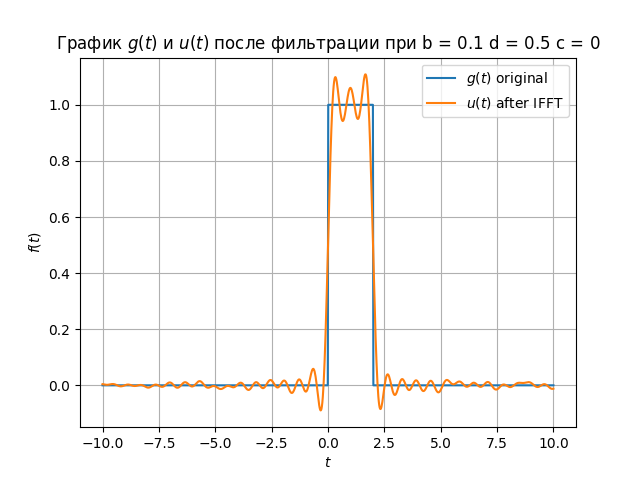
\includegraphics[width=1\linewidth]{pic/f_0.1_10.png}\\а)}
\end{minipage}
\hfill
\begin{minipage}[h]{0.5\linewidth}
\center{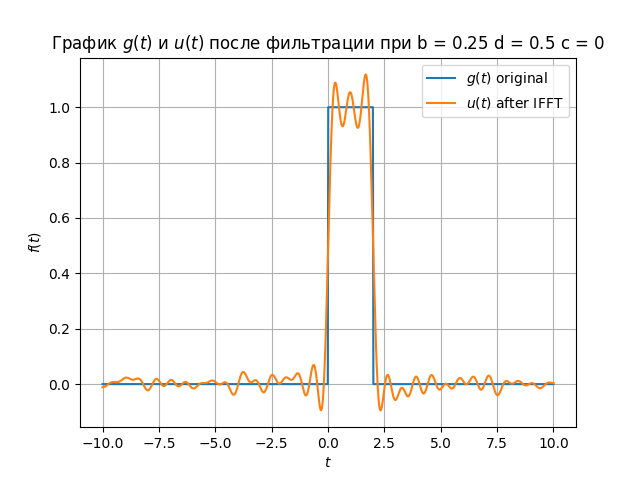
\includegraphics[width=1\linewidth]{pic/f_0.25_10.png}\\б)}
\end{minipage}
\caption{Сигнал $g(t)$ и $u(t)$ после фильтрации при $\nu_0 = 10$ а) $b=0.1$, б) $b=0.25$.}

\begin{minipage}[h]{0.5\linewidth}
\center{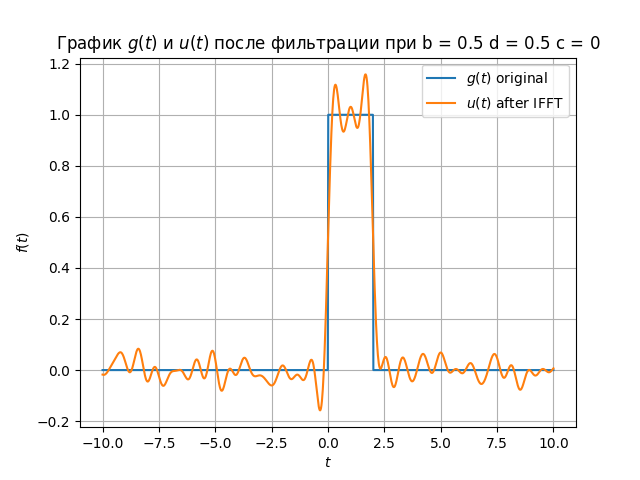
\includegraphics[width=1\linewidth]{pic/f_0.5_10.png}\\а)}
\end{minipage}
\hfill
\begin{minipage}[h]{0.5\linewidth}
\center{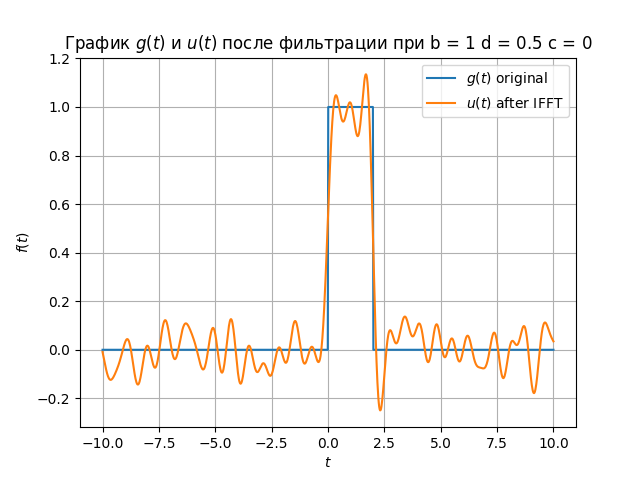
\includegraphics[width=1\linewidth]{pic/f_1_10.png}\\б)}
\end{minipage}
\caption{Сигнал $g(t)$ и $u(t)$ после фильтрации при $\nu_0 = 10$ а) $b=0.5$, б) $b=1$.}
\end{figure}

\newpage
 При увеличении параметра $b$ в уравнении, задающем шумы, снижается эффективность фильтрации. Это происходит, потому что чем больше значение $b$, тем больше шумов добавляется к исходной функции $g(t)$. При увеличении параметра $\nu_0$ полученная после фильтрации картинка становится четче и ближе к исходной функции $g(t)$.






\subsection{Убираем специфические частоты}

Пусть $b = 0.5, c = 0.5, d = 5$. Найдем Фурье-образ сигнала.

\begin{figure}[h!]
\center{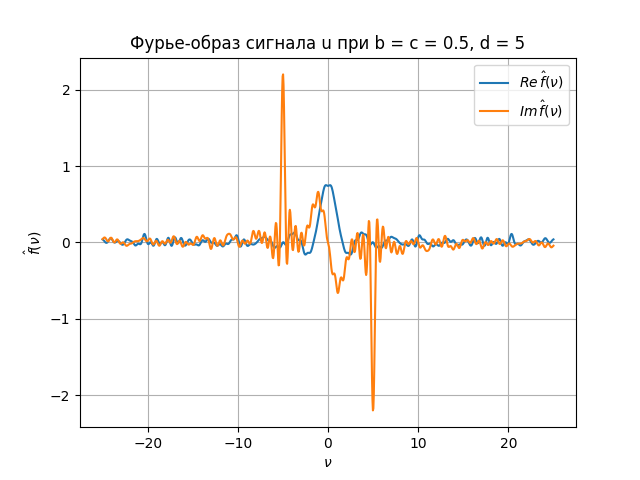
\includegraphics[width=1\linewidth]{pic/s_0.5_0.5_5.png}}
\caption{Фурье-образ функции $u(t)$ при $b = 0.5, c = 0.5, d = 5$.}
\end{figure}

\newpage
Попробуем убрать сначала высокие частоты, с помощью обнуления определенного диапазона частот, возьмем $\nu_0 = 10$ и воспользуемся способом из пункта 1.1.


\begin{figure}[h!]
\center{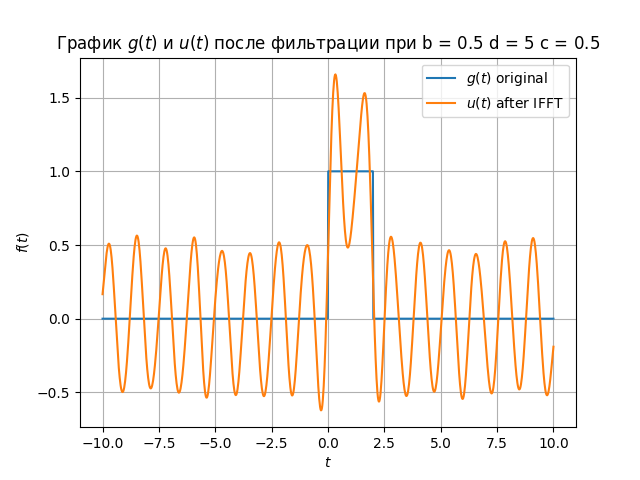
\includegraphics[width=0.7\linewidth]{pic/s_res_0.5_0.5_5.png}}
\caption{Функция $g(t)$ при $b = 0.5, c = 0.5, d = 5$  и $u(t)$ без высоких частот.}
\end{figure}

Получим график (рисунок 17), в котором теперь основной шум представляют гармонические колебания. Попробуем обнулить частоты, которым соответствуют наибольшие скачки функции $Im \hat{f}(\nu)$ (рисунок 16), то есть около 5 и -5.

\begin{figure}[h!]
\center{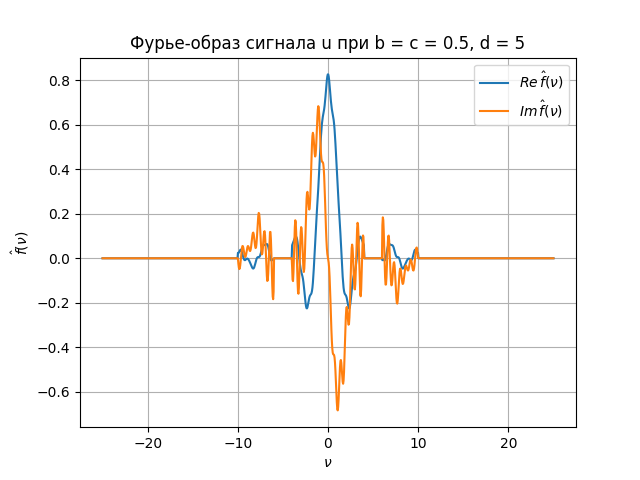
\includegraphics[width=0.8\linewidth]{pic/s_im_res_0.5_0.5_5.png}}
\caption{Фурье-образ функции $u(t)$ при $b = 0.5, c = 0.5, d = 5$ после фильтрации.}
\end{figure}



\begin{figure}[h!]
\center{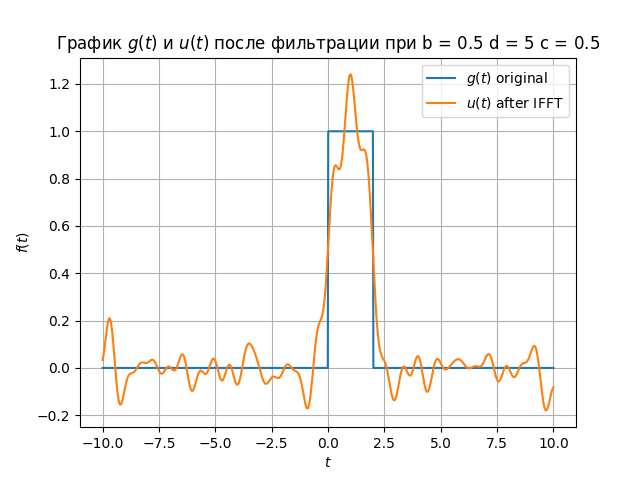
\includegraphics[width=0.7\linewidth]{pic/s_res.png}}
\caption{Функция $g(t)$ при $b = 0.5, c = 0.5, d = 5$  и $u(t)$ после фильтрации от высоких частот и от специальных.}
\end{figure}




\begin{figure}[h!]
\begin{minipage}[h]{0.5\linewidth}
\center{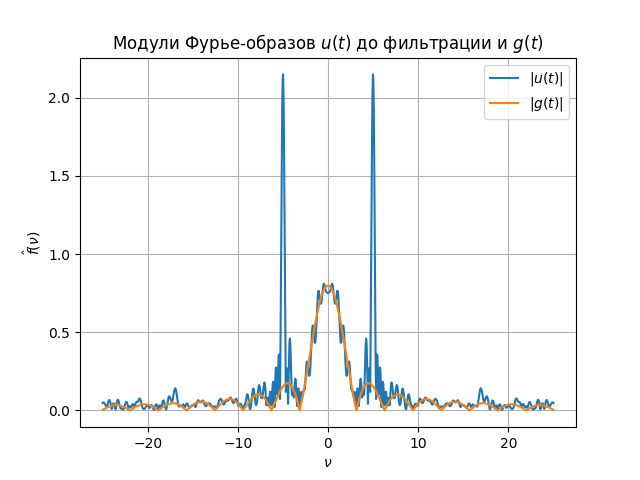
\includegraphics[width=1\linewidth]{pic/s_abs_start.png}\\а)}
\end{minipage}
\hfill
\begin{minipage}[h]{0.5\linewidth}
\center{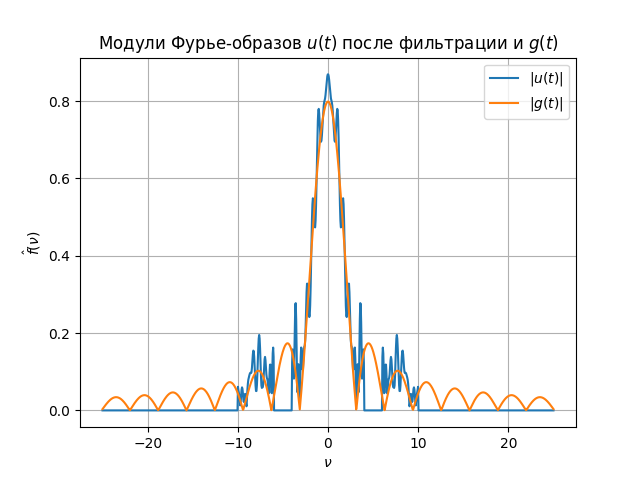
\includegraphics[width=1\linewidth]{pic/s_abs_res.png}\\б)}
\end{minipage}
\caption{Модули образов $g(t)$ и сигнала $u(t)$ до фильтрации (а) и после(б).}
\end{figure}

\newpage
В результате получаем график, изображенный на рисунке 19, шумы, присутствующие ранее заметно снизились и теперь $u(t)$ лучше приближает исходную функцию $g(t)$.\\
%Исследуем влияние частот среза и значений параметров $b, c, d$ на вид помех и эффективность фильтрации.



\newpage
\subsection{Убираем низкие частоты?}
Рассмотрим фильтр, который обнуляет Фурье-образ на всех частотах в некоторой окрестности точки $\nu = 0$.

\begin{figure}[h!]
\center{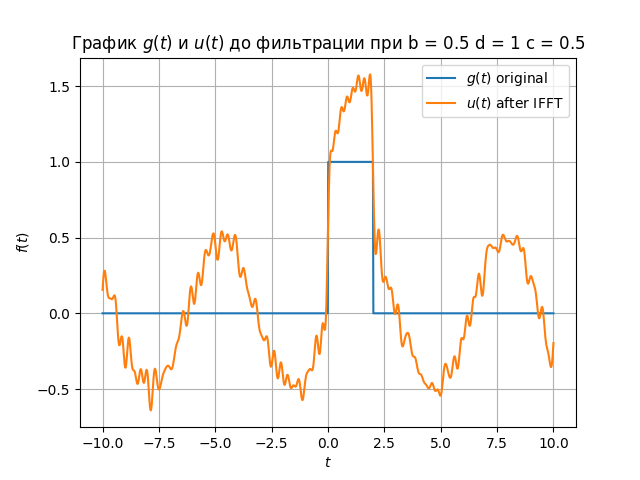
\includegraphics[width=0.65\linewidth]{pic/l_st.png}}
\caption{Функция $g(t)$ при $b = 0.5, c = 0.5, d = 1$  и $u(t)$ до фильтрации.}
\end{figure}

\begin{figure}[h!]
\center{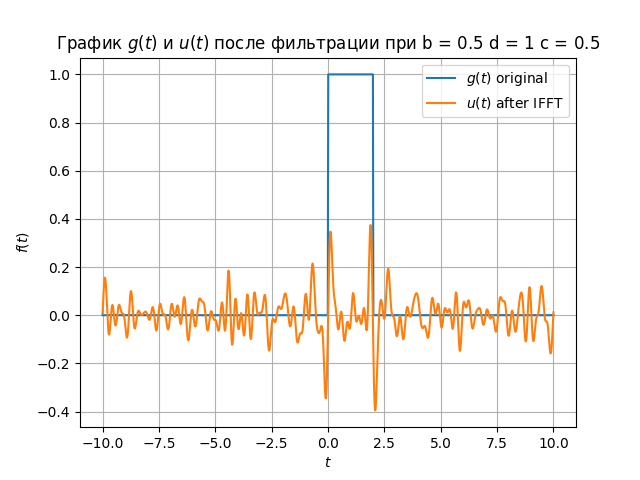
\includegraphics[width=0.7\linewidth]{pic/l_aft_5.png}}
\caption{Функция $g(t)$ при $b = 0.5, c = 0.5, d = 1$  и $u(t)$ после фильтрации $|\nu | < 5$.}
\end{figure}

Заметим, что фильтр снизил амплитуду гармонической составляющей помех, но вместе с ней понизилось и сходство с графиком исходной функции (рисунок 22).\\ 

 Рассмотрим влияние изменения ширины промежутка, в котором мы зануляем частоты.


\begin{figure}[h!]
\begin{minipage}[h]{0.5\linewidth}
\center{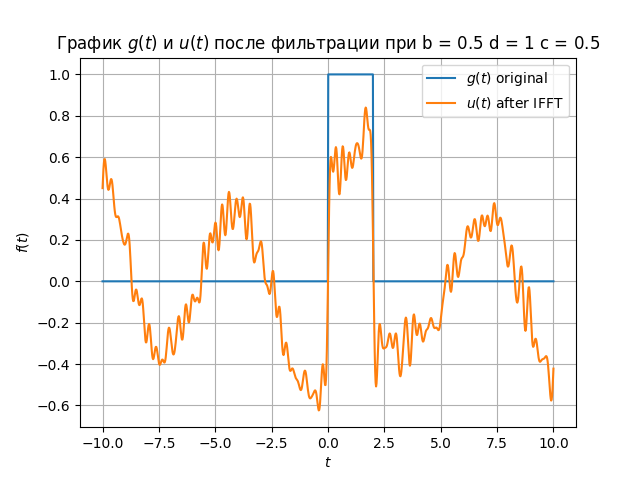
\includegraphics[width=1\linewidth]{pic/l_1.png}\\а)}
\end{minipage}
\hfill
\begin{minipage}[h]{0.5\linewidth}
\center{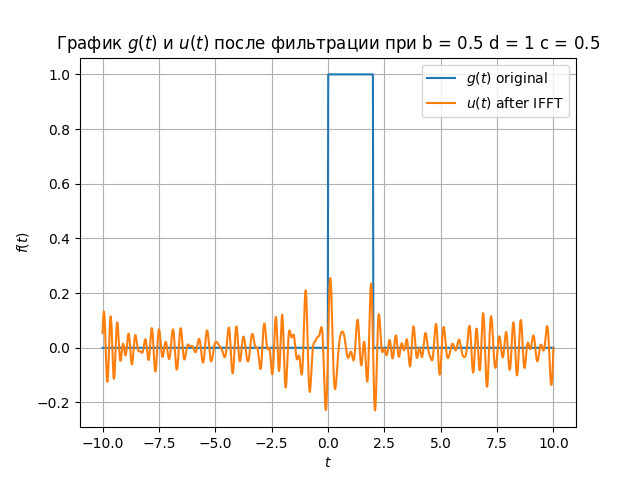
\includegraphics[width=1\linewidth]{pic/l_10.png}\\б)}
\end{minipage}
\caption{Графики $g(t)$ и сигнала $u(t)$ после фильтрации при а) $|\nu| < 1$ и б) $|\nu| < 10$.}
\end{figure}

На рисунках 22-23 заметно, что при увеличении промежутка снижется количество шумов, но пропадает и нужный нам сигнал. В нашем случае фильтрация низких частот оказалась малоэффективной при любом промежутке $[-\nu, \nu]$.



\newpage
\section{Задание. Фильтрация звука.}



%Для визуализации был написан код на языке \textit{Python}. \\
%Код расположен на \href{https://github.com/a-nechaeva/practical_Linal/tree/main/lab4}{\textbf{GitHub}}.


\end{document}













